\documentclass[a4paper]{article}
\addtolength{\hoffset}
{-2.25cm}
\addtolength{\textwidth}
{5cm}
\addtolength{\voffset}
{-3.25cm}
\addtolength{\textheight}
{5.5cm}
\setlength{\parskip}{0pt}
\setlength{\parindent}{0in}

\usepackage[utf8]{inputenc}
\usepackage{microtype}
\usepackage[english]{babel}
\usepackage{fancyhdr}
\usepackage{advdate}
\usepackage{enumitem}
\usepackage{amsmath, amssymb}
\usepackage{graphicx}
\usepackage{caption}
\usepackage{subcaption}
\usepackage{float}
\usepackage{titlesec}
\usepackage{wasysym}
\usepackage{url}
\usepackage{hyperref}
\usepackage{tikz, verbatimbox}
\usepackage{fixltx2e}
\usepackage{centernot}
\usepackage{algorithm}
\usepackage{algpseudocode}
\usepackage{listings}
\usetikzlibrary{shapes.geometric, arrows}
\usetikzlibrary{positioning}
\usepackage[table]{xcolor}

\graphicspath{{./static/}}
\tikzset{every picture/.style={line width=0.75pt}} %set default line width to 0.75pt

\newcommand{\LComment}[1]{\State \(\triangleright\) \text{#1}}
\MakeRobust{\Call}

\begin{document}

\fancyhead[c]{}
\hrule \medskip
\begin{minipage}{0.195\textwidth}
\raggedright
Rishabh Indoria\\
21F3001823
\end{minipage}
\begin{minipage}{0.6\textwidth}
\centering
\LARGE
Reinforcement Learning
\end{minipage}
\begin{minipage}{0.195\textwidth}
\raggedleft
\today \hfill \\
\end{minipage}
\medskip \hrule
\bigskip

\section{Introduction to Reinforcement Learning}
\begin{itemize}
    \item A trial and error learning paradigm, rewards and punishments.
    \item Learn about a system through interaction.
    \item The idea is inspired by behavioral psychology.
    \item We use RL when the system has complex dynamics, we have a complex workspace
    \item Stochastic sensing and actuation is required
    \item Human-in-the-loop learning
    \item Customization/Personalization, Recommendation systems
    \item RL goes beyond human knowledge, it can learn through self play.
    \item RL can be used to improve heuristics.
    \item Book to be used is "Reinforcement Learning: An Introduction", $2^{nd}$ edition, this can be found \href{https://www.andrew.cmu.edu/course/10-703/textbook/BartoSutton.pdf}{here}.\label{Book}
\end{itemize}

\section{Fundamental Concepts in RL}
\subsection{Games and Learning}
\begin{itemize}
    \item Consider the game of Tic-tac-toe
    \item We can set up a supervised learning paradigm based on current position and the correct move.
    \item Then we can use any model to train and predict the move.
    \item In RL we learn from evaluation, so if the model wins then it gets $1$ point, if it loses then it gets $-1$ point and if it draws then it gets $0$ points.
    \item RL will learn from repeated play.
    \item \textbf{MENACE}: Matchbox based learning for tic-tac-toe.
    \item Each matchbox has a position drawn on it, and inside it are different colored beads which correspond to different moves the computer/matchbox can make.
    \item Let's say we play a game, then we would have chosen some number of matchboxes and picked some beads.
    \item If matchbox wins then add two of the beads back in the matchbox, and if it looses then we throw away the beads.
    \item By doing this, we are essentially increasing the probability of winning for the matchbox.
    \item We had to wait till the end of the game to update, but we don't need to wait till the end, we can check intermediate states based on some rules.
    \item We can also remember previous plays and say that a certain position has a higher or lower chance of winning. Now, for every move, we would want the chance of winning to go up.
    \item \textbf{Temporal Difference Learning}: Look at successive states and change action probabilities based on chance of winning.
    \item TD is a simple rule to explain complex behaviors.
    \item \textbf{Intuition}: Prediction of outcome at time $t+1$ is better than the prediction at time $t$. Hence, use the later prediction to adjust the earlier prediction.
\end{itemize}

\subsection{Bandit Problems}
\begin{itemize}
    \item At the core of RL is exploration vs exploitation.
    \item \textbf{Immediate Reinforcement}: The payoff accrues immediately after an action is chosen.
    \item One key question they try to solve is the dilemma between exploration vs exploitation.
    \item \textbf{Bandit problems} encapsulate 'Explore vs Exploit'.
    \item We are trying to find profitable actions.
    \item We exploit to act according to the best observations already made.
    \item Always exploring might not be optimal, always exploiting might not be optimal either. 
    \item \textbf{Multi-arm Bandits}: $n$-arm bandit problem is to learn to preferentially select a particular action(arm) from a set of actions $(1,2,3,...,n)$.
    \item Each selection results in Rewards derived from the respective probability distribution.
    \item Arm $i$ has a reward distribution with mean $\mu_i$ and $\mu^*=\max\{\mu_i\}$.
    \item We are trying to identify the arm with mean $\mu^*$.
    \item Objective is to identify the correct arm eventually.
    \item We first look at traditional approaches
    \item Let $r_{i,k}$ be the reward sample acquired when $i^{th}$ arm is selected for the $k^{th}$ time.
    \item $Q(a_i)$ is the average or expected reward that we get by choosing $a_i$.
    \item Define
    \begin{equation*}
        \begin{split}
            &Q(a_i)=\frac{\sum_kr_{i,k}}{\sum_{\{k:r_{i,k}\}}1}\text{\quad}Q(a^*)=\max\{Q(a_i)\}\\
            &Q_{k+1}(a_i)=Q_k(a_i)+\alpha (r_{i,k}-Q_k(a_i))
        \end{split}
    \end{equation*}
    \item Setting $\alpha=\frac{1}{k_i+1}$ yields the average.
    \item Setting $\alpha$ to a constant makes the expression a weighted average.
    \item \textbf{Epsilon Greedy}: Select arm $a^*=\argmax_i\{Q_k(a_i)\}$ with probability $1-\epsilon$ and select any arbitrary arm with probability $\epsilon$. Usually $\epsilon$ is very small.
    \item This is an exploration method, works fairly well in real world scenarios.
    \item \textbf{Softmax}: Select arms with probability proportional to the current value estimates
    \begin{equation*}
        \pi_k(a_i)=\frac{\exp{(Q_k(a_i)/\tau)}}{\sum_j\exp{(Q_k(a_j)/\tau)}}
    \end{equation*}
    \item $\tau$ is called temperature, low temperature corresponds to greedy or exploitation and high temperature corresponds to uniform or exploration.
\end{itemize}

\subsection{Regret and PAC Frameworks}
\begin{itemize}
    \item So far, we maximized the total rewards obtained
    \item But we can also try to minimize \textbf{regret}(loss) while learning.
    \item We can also use \textbf{Probably Approximately Correct} frameworks(PAC)
    \begin{enumerate}
        \item Identification of an $\epsilon$-optimal arm with probability $1-\delta$
        \item $\epsilon$-optimal: Mean of the selected arm satisfies
        \begin{equation*}
            \mu>\mu^*-\epsilon
        \end{equation*}
        \item Minimize sample complexity: Order of samples required for such an arm identification.
    \end{enumerate}
    \item Practical algorithms tend to go the regret route rather than PAC optimality.
    \item \textbf{Median Elimination} achieves PAC optimality, it is a round based algorithm.
    \item Due to this algorithm, more and more algorithms are developed based on round based method.
    \item \textbf{Upper Confidence Bounds} achieves regret optimality, idea is to reduce the constants hidden in big $O$ notation.
    \item The arm with the best estimate $r^*$ so far serves as a benchmark, and other arms are played only if the upper bound of a suitable confidence interval is at least $r^*$.
    \item \textbf{Simple Approach}: Be greedy with respect to upper confidence bounds.
    \item Sub-optimal arm $j$ is played fewer than $(8/\Delta_j)$ in $n$ times.
    \item Consider a deterministic policy $UCB1$
    \item \textbf{Initialization}: Play each arm once.
    \item \textbf{Loop}: Play arm $j$ that maximizes $\Bar{x}_j+\sqrt{\frac{2\ln{n}}{n_j}}$ where $\Bar{x}_j$ is the average reward obtained from arm $j$, $n_j$ is the number of times arm $j$ has been played so far, and $n$ is the overall number of plays done so far.
    \item Details regarding this algorithm can be found in \href{https://homes.di.unimi.it/~cesabian/Pubblicazioni/ml-02.pdf}{this paper}.
    \item \textbf{Thompson Sampling} also achieves regret optimality, this is a Bayesian approach.
\end{itemize}

\subsection{Contextual Bandits}
\begin{itemize}
    \item Different ads for different users, we can use one bandit for each user.
    \item However, this is hard to train, needs several rounds of experience with same user.
    \item Assume that the parameters of the reward distributions themselves are determined by a set of hyperparameters.
    \\item Typical assumption is a linear parameterization of the expectation.
    \item Essentially grouping users based on some context, age, gender, last queries, etc.
    \item Assume that each user is represented by a set of features, can be joint features of user and arm.
    \item The "static" used for choosing arms is now dependent on these features.
    \item Could correspond to the presence or absence of different signals.
    \item We could also have features for arms, in case there are way too many arms.
    \item \textbf{LinUCB} is one of the more popular contextual bandit algorithms, whose \href{https://arxiv.org/pdf/1003.0146}{paper can be found here}.
    \item Idea is that \textbf{Predicted expected reward} is assumed to be a linear function of the features.
    \begin{enumerate}
        \item Use ridge regression to fit parameters
        \item Can derive an upper confidence bounds for the regression fit
        \item Use UCB like action selection
        \item Gives better performance with lesser "training" data
    \end{enumerate}
    \item Bandits have only actions
    \item Contextual bandits have actions, context, but no sequence.
    \item A full RL problem will have all three.
    \item I have implemented multiple methods for the multi armed bandit problem, which can be found at \url{https://colab.research.google.com/drive/15vgC170tQthc2DVUM3ZN_-jqJiyclGHl?usp=sharing}
\end{itemize}

\subsection{Full RL Problem}
\begin{itemize}
    \item Action at a Temporal Distance
    \item Learning an appropriate action at state $1$ is dependent on the actions at future states.
    \item There is \textbf{no immediate} feedback.
    \item We have an agent and environment.
    \item Learn from close interaction with a stochastic environment having noisy delayed scalar evaluation with a goal to maximize a measure of long term performance.
    \begin{figure}[H]
        \centering
        \includegraphics[width=0.5\linewidth]{Degree//static/RL_simple_framework.png}
        \caption{Simplified RL framework}
    \end{figure}
    \item Bandit problem can be viewed as having a single state, and multiple actions that lead to certain rewards.
    \begin{figure}[H]
        \centering
        \begin{subfigure}[b]{0.45\textwidth}
            \centering
            \includegraphics[width=0.7\textwidth]{Degree/static/RL_bandit_problem.png}
            \caption{Bandit Problem}
        \end{subfigure}
        \hfill
        \begin{subfigure}[b]{0.45\textwidth}
            \centering
            \includegraphics[width=0.7\textwidth]{Degree/static/RL_contextual_bandit_problem.png}
            \caption{Contextual Bandit Problem}
        \end{subfigure}
    \end{figure}
    \item \textbf{Idea}: Use prediction as \textbf{surrogate} feedback. This allows us to get immediate reward.
\end{itemize}

\section{Markov Decision Processes}
\subsection{Introduction to MDP}
\begin{itemize}
    \item Putting together the complete RL problem, we define the \textbf{Agent-Environment Interface}.
    \begin{figure}[H]
        \centering
        \includegraphics[width=0.5\linewidth]{Degree//static/RL_agent_environment_interface.png}
        \caption{The Agent-Environment Interface}
    \end{figure}
    \item Agent and Environment interact at discrete time steps: $t=0,1,2,...$
    \item Agent observes state at step $t$: $s_t\in S$
    \item produces action at step $t$: $a_t\in A(s_t)$
    \item gets resulting reward: $r_{t+1}\in \mathcal{R}$
    \item and resulting next state: $S_{t+1}$
    \begin{figure}[H]
        \centering
        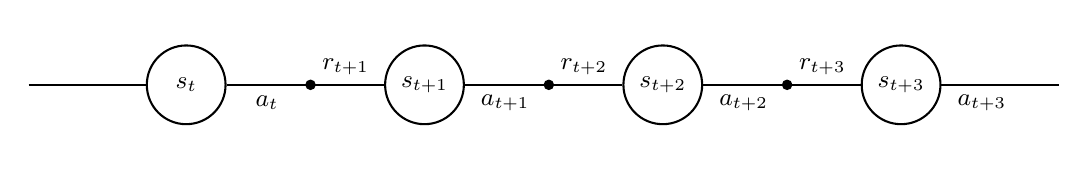
\begin{tikzpicture}[every node/.style={draw, circle, minimum size=1cm, font=\small}, node distance=1.5cm]
            % States
            \node (s0) {$s_t$};
            \node[right=2cm of s0] (s1) {$s_{t+1}$};
            \node[right=2cm of s1] (s2) {$s_{t+2}$};
            \node[right=2cm of s2] (s3) {$s_{t+3}$};
            
            % Actions
            \node[below right=-0.5cm and 0.3cm of s0, draw=none] (a0) {$a_t$};
            \node[below right=-0.5cm and 0.3cm of s1, draw=none] (a1) {$a_{t+1}$};
            \node[below right=-0.5cm and 0.3cm of s2, draw=none] (a2) {$a_{t+2}$};
            \node[below right=-0.5cm and 0.3cm of s3, draw=none] (a3) {$a_{t+3}$};
            
            % Rewards
            \node[above right=-0.5cm and 1.3cm of s0, draw=none] (r1) {$r_{t+1}$};
            \node[above right=-0.5cm and 1.3cm of s1, draw=none] (r2) {$r_{t+2}$};
            \node[above right=-0.5cm and 1.3cm of s2, draw=none] (r3) {$r_{t+3}$};
        
            % Black dots
            \node[right=1cm of s0, draw, fill=black, circle, minimum size=3pt, inner sep=0pt] (b0) {};
            \node[right=1cm of s1, draw, fill=black, circle, minimum size=3pt, inner sep=0pt] (b1) {};
            \node[right=1cm of s2, draw, fill=black, circle, minimum size=3pt, inner sep=0pt] (b2) {};
            
            % Draw edges
            \draw[-] (-2,0) -- (s0);
            \draw[-] (s0) -- (s1);
            \draw[-] (s1) -- (s2);
            \draw[-] (s2) -- (s3);
            \draw[-] (s3) -- ++(2,0);
        \end{tikzpicture}
        \caption{Rolled out Interface}
    \end{figure}
    \item "the state" at step $t$, means whatever information is available to the agent at step $t$ about its environment.
    \item The state can include immediate "sensations", highly processed sensations, and structures built up over time from sequences of sensations.
    \item Ideally, a state should summarize past sensations to retain all "essential" information, i.e., it should have the \textbf{Markov Property}
    \begin{equation*}
        Pr\{s_{t+1}=s',r_{t+1}=r|s_t,a_t,r_t,s_{t-1},a_{t-1},r_{t-1},...\}=Pr\{s_{t+1}=s',r_{t+1}=r|s_t,a_t,r_t\}\text{ }\forall s',r
    \end{equation*}
    \item \textbf{Markov Decision Processes}, $M$, is the tuple: $M=\langle S,A,p,r\rangle$
    \begin{enumerate}
        \item $S$: set of states
        \item $A$: set of actions
        \item $p$: $S\times A\times S\to [0,1]$, probability of transition
        \item $r$: $S\times A\times S\to \mathbb{R}$, expected reward
    \end{enumerate}
    \item Goal of the agent is to learn an \textbf{optimal} policy $\pi:S\times A\to [0,1]$, can be deterministic.
    \item We want to learn a policy such that expected reward is maximized.
    \item The policy that achieves maximum total expected reward is the \textbf{optimal} policy.
    \item \textbf{States}: Enough information to take decisions, Raw inputs, are often not sufficient.
    \item \textbf{Actions}: The control variables, can be discrete or continuous.
    \item \textbf{Rewards}: Defines the goal of the problem.
\end{itemize}

\subsection{Returns and Value Functions}
\begin{itemize}
    \item \textbf{Policy} at step $t$, $\pi_t$: A mapping from states to action probabilities,\\
    $\pi_t(s,a)=$ probability that $a_t=a$ when $s_t=s$
    \item Reinforcement learning methods specify how the agent changes its policy as a result of experience.
    \item Roughly, the agent's goal is to get as much reward as it can over the long run.
    \item Suppose the sequence of rewards after step $t$ is: $r_{t+1},r_{t+2},r_{t+3},...$
    \item We want to maximize the \textbf{return}, $G_t$, for each step $t$.
    \item \textbf{Episodic tasks}: Interaction breaks naturally into episodes, have some end point, e.g., plays of a game, trips through a maze.
    \begin{equation*}
        G_t=r_{t+1}+r_{t+2}+...+r_T
    \end{equation*}
    where $T$ is a final time step at which a \textbf{terminal state} is reached, ending an episode.
    \item \textbf{Continuous tasks}: Interaction does not have natural episodes. In this case we use \textbf{Discounted return}
    \begin{equation*}
        G_t=r_{t+1}+\gamma r_{t+2}+\gamma^2r_{t+3}+...=\sum_{k=0}^\infty \gamma^kr_{t+k+1}
    \end{equation*}
    where $\gamma,0\leq \gamma \leq 1$, is the \textbf{discount rate}. shortsighted $0\gets \gamma \to 1$ farsighted.
    \item In general, we want to maximize the \textbf{expected return}, $E\{G_t\}$, for each step $t$.
    \item If we are sure that states will end at some point then take $\gamma=1$ else $\gamma$ is strictly less than $1$.
    \item \textbf{Value Functions}: Expected future rewards, starting at a state or state-action pair and following policy $\pi$.
    \item \textbf{State-value function for policy $\pi$}
    \begin{equation*}
        v_\pi(s)=E_\pi[\sum_{k=0}^\infty \gamma^kR_{t+k+1}|S_t=s]=E_\pi[G_t|S_t=s]
    \end{equation*}
    \item \textbf{Action-value function for policy $\pi$}
    \begin{equation*}
        q_\pi(s,a)=E_\pi[\sum_{k=0}^\infty \gamma^kR_{t+k+1}|S_t=s,A_t=a]=E_\pi[G_t|S_t=s,A_t=a]
    \end{equation*}
    \item Both of these are connected as follows
    \begin{equation*}
        v_\pi(s)=\sum_a\pi(a|s)q_\pi(s,a)=E_\pi[q_\pi(s,a)]
    \end{equation*}
    \item We can use either but $q_\pi$ ends up being better than $v_\pi$ in a lot of the problems.
\end{itemize}

\section{Stochastic Dynamic Programming}
\subsection{Bellman Equations}
\begin{itemize}
    \item \textbf{Bellman Equation for a Policy $\pi$}
    \begin{equation*}
        \begin{split}
            v_\pi(s)=&E_\pi[G_t|S_t=s]\\
            =&E_\pi[R_{t+1}+\gamma G_{t+1}|S_t=s]\\
            =&\sum_a\pi(a|s)\sum_{s'}\sum_rp(s',r|s,a)[r+\gamma E_\pi[G_{t+1}|S_{t+1}=s']]\\
            =&\sum_a\pi(a|s)\sum_{s',r}p(s',r|s,a)[r+\gamma v_\pi(s')],\text{ for all }s\in \mathcal{S}
        \end{split}
    \end{equation*}
    \item From $s$ we can take a number of actions based on policy $\pi$
    \item For each action, there could be a number of states that it could lead and their corresponding reward.
    \item We can write $E_\pi[G_{t+1}|S_{t+1}=s']=E_\pi[G_t|S_t=s']=v_\pi(s')$ because of Markov property and stationary.
    \item This is a linear equation in $\lvert S\rvert$ variables.
    \item A unique solution for this exists.
    \item \textbf{Equiprobable Random Policy}: Same probability for all actions.
    \item For finite MDPs, policies can be partially ordered.
    \item $\pi \geq \pi'$ if and only if $v_\pi(s)\geq v_{\pi'}(s)$ for all $s\in \mathcal{S}$
    \item There is always at least one (possibly many) policies that is better than or equal to all the others. This is an \textbf{optimal policy}. We denote them all as $\pi^*$
    \item There is at least one policy that is deterministic.
    \item Optimal policies share the same optimal state-value function
    \begin{equation*}
        \begin{split}
            &v_{*}(s)=\max_\pi v_\pi(s)\text{ for all }s\in \mathcal{S}\\
            &q_{*}(s,a)=\max_\pi q_\pi(s,a)\text{ for all }s\in \mathcal{S}\text{ and }a\in \mathcal{A}
        \end{split}
    \end{equation*}
    \item Try to derive optimal value function, from this derive the optimal policy.
    \item \textbf{Bellman Optimality Equation for $v_*$}: The value of a state under an optimal policy must equal the expected return for the best action from that state.
    \begin{equation*}
        \begin{split}
            v_*(s)=&\max_{a\in \mathcal{A}(s)}q_{\pi^*}(s,a)\\
            =&\max_aE_{\pi^*}[G_t|S_t=s,A_t=a]\\
            =&\max_aE_{\pi^*}[R_{t+1}+\gamma G_{t+1}|S_t=s,A_t=a]\\
            =&\max_aE[R_{t+1}+\gamma v_*(S_{t+1})|S_t=s,A_t=a]\\
            =&\max_a\sum_{s',r}p(s',r|s,a)[r+\gamma v_*(s')]
        \end{split}
    \end{equation*}
    \item \textbf{Bellman Optimality Equation for $q_*$}
    \begin{equation*}
        \begin{split}
            q_*(s,a)=&E_{\pi*}[G_t|S_t=s,A_t=a]\\
            =&E_{\pi^*}[R_{t+1}+\gamma G_{t+1}|S_t=s,A_t=a]\\
            =&E[R_{t+1}+\gamma v_*(S_{t+1})|S_t=s,A_t=a]\\
            =&E[R_{t+1}+\gamma \max_{a'}q_*(S_{t+1},a')|S_t=s,A_t=a]\\
            =&\sum_{s',r}p(s',r|s,a)[r+\gamma \max_{a'}q_*(s',a')]
        \end{split}
    \end{equation*}
    \item Any policy that is greedy with respect to $v_*$ is an optimal policy.
    \item Therefore, given $v_*$, one-step lookahead search produces the long-term optimal actions.
    \item Given $q_*$, the agent does not even have to do a one-step lookahead search.
    \begin{equation*}
        \pi_*(s)=\argmax_{a\in \mathcal{A}(s)}q_*(s,a)
    \end{equation*}
\end{itemize}

\subsection{Policy and Value Iteration}
\begin{itemize}
    \item DP is the solution method of choice for MDPs
    \item Requires complete knowledge of system dynamics(transition matrix and rewards), Computationally expensive, Curse of dimensionality however it is guaranteed to converge.
    \item \textbf{Policy Iteration}: We solve for $v_\pi$ iteratively using its bellman equation.
    \item We keep iterating until $v_{k+1}$ and $v_{k}$ are sufficiently close.
    \begin{algorithm}[H]
        \caption{Iterative Policy Evaluation Algorithm}
        \begin{algorithmic}[1]
            \Statex Input $\pi$, the policy to be evaluated
            \Statex Algorithm parameter: A small threshold $\theta>0$ determining accuracy of estimation.
            \State Initialize $V(s)$, for all $s\in \mathcal{S}^+$, arbitrarily except that $V(terminal)=0$
            \Repeat
                \State $\Delta \gets 0$
                \For{each $s\in \mathcal{S}$}
                    \State $v\gets V(s)$
                    \State $V(s)\gets \sum_a\pi(a|s)\sum_{s',r}p(s',r|s,a)[r+\gamma V(s')]$
                    \LComment If $s'$ is terminal state then replace $[r+\gamma V(s')]$ with $[r]$
                    \State $\Delta \gets \max(\Delta,\lvert v-V(s)\rvert)$
                \EndFor
            \Until{$\Delta<\theta$}
        \end{algorithmic}
    \end{algorithm}
    \item One issue or feature of the above algorithm is that once $V(s_1)$ is updated, then all other states will use the updated value rather than the previous value.
    \item Suppose we have computed $v_\pi$ for an arbitrary deterministic policy $\pi$.
    \item The value of doing $a$ in state $s$ is
    \begin{equation*}
        \begin{split}
            q_\pi(s,a)=&E[R_{t+1}+\gamma v_\pi(S_{t+1})|S_t=s,A_t=a]\\
            =&\sum_{s',r}p(s',r|s,a)[r+\gamma v_\pi(s')]
        \end{split}
    \end{equation*}
    \item It is better to switch to action $a\neq \pi(s)$ for state $s$ if and only if $q_\pi(s,a)>v_\pi(s)=q_\pi(s,\pi(s))$
    \item Doing this for all states to get a new policy $\pi'$ that is greedy with respect to $v_\pi$
    \begin{equation*}
        \begin{split}
            \pi'(s)=&\argmax_aq_\pi(s,a)\\
            =&\argmax_a\sum_{s',r}p(s',r|s,a)[r+\gamma v_\pi(s')]
        \end{split}
    \end{equation*}
    \item This will guarantee $v_{\pi'}\geq v_\pi$
    \item If we keep doing this then at some point we will find $v_{\pi'}=v_\pi$ for all states
    \begin{equation*}
        v_{\pi'}(s)=\max_a\sum_{s',r}p(s',r|s,a)[r+\gamma v_\pi(s')]
    \end{equation*}
    \item But this is the Bellman Optimality Equation
    \item So, $v_{\pi'}=v_*$ and both $\pi$ and $\pi'$ are optimal policies.
    \item \textbf{Policy Iteration}: $\pi_0\xrightarrow{E}v_{\pi_0}\xrightarrow{I}\pi_1\xrightarrow{E}v_{\pi_1}\xrightarrow{I}\pi_2\xrightarrow{E}...\xrightarrow{I}\pi_*\xrightarrow{E}v_*$\\
    $E$ corresponds to policy evaluation, $I$ corresponds to policy improvement, "greedification".
    \begin{algorithm}[H]
        \caption{Policy Iteration Algorithm}
        \begin{algorithmic}[1]
            \LComment 1. Initialization
            \State $V(s)\in \mathbb{R}$ and $\pi(s)\in \mathcal{A}(s)$ arbitrarily for all $s\in \mathcal{S}$
            \Statex
            \Loop
                \LComment 2. Policy Evaluation
                \Repeat
                    \State $\Delta \gets 0$
                    \For{each $s\in \mathcal{S}$}
                        \State $v\gets V(s)$
                        \State $V(s)\gets \sum_{s',r}p(s',r|s,\pi(s))[r+\gamma V(s')]$
                        \LComment Again if $s'$ is terminal, then replace $[r+\gamma V(s')]$ with $[r]$
                        \State $\Delta \gets \max(\Delta,\lvert v-V(s)\rvert)$
                    \EndFor
                \Until{$\Delta<\theta$}
                \Statex
                \LComment 3. Policy Improvement
                \State $policy\text{-}stable\gets true$
                \For{each $s\in \mathcal{S}$}
                    \State $old\text{-}action\gets \pi(s)$
                    \State $\pi(s)\gets \argmax_a\sum_{s',r}|p(s',r|s,a)[r+\gamma v_\pi(s')]$
                    \LComment Break ties consistently so that we don't oscillate between ties.
                    \If{$old\text{-}action\neq \pi(s)$}
                        \State $policy\text{-}stable\gets false$
                    \EndIf
                \EndFor
                \If{$policy\text{-}stable$}
                    \State \Return $V\approx v$, and $\pi \approx \pi_*$
                \EndIf
            \EndLoop
        \end{algorithmic}
    \end{algorithm}
    \item The above algorithms utilize the bellman optimality equation for action-value function.
    \item We can also use the equation for state-value function.
    \item state-value function can be updated iteratively without having to calculate policy at each iteration.
    \item We will calculate deterministic policy only once, at the end of the loop.
    \item \textbf{Value Iteration Algorithm}
    \begin{algorithm}[H]
        \caption{Value Iteration Algorithm}
        \begin{algorithmic}[1]
            \Statex Algorithm parameters: A small threshold $\theta>0$ determining accuracy of estimation.
            \Statex Initialize $V(s)$, for all $s\in \mathcal{S}^+$ arbitrarily except that $V(terminal)=0$
            \Repeat
                \State $\Delta \gets 0$
                \For{each $s\in \mathcal{S}$}
                    \State $v\gets V(s)$
                    \State $V(s)\gets \max_a{\sum_{s',r}p(s',r|s,a)[r+\gamma V(s')]}$
                    \State $\Delta \gets \max{(\Delta,\lvert v-V(s)\rvert)}$
                \EndFor
            \Until{$\Delta<\theta$}
            \Statex Output a deterministic policy, $\pi \approx \pi_*$ such that
            \State $\pi(s)=\argmax_a\sum_{s',r}p(s',r|s,a)[r+\gamma V(s')]$
        \end{algorithmic}
    \end{algorithm}
    \item In these algorithms, we have to do the updates over the entire state set.
\end{itemize}

\subsection{Asynchronous Dynamic Programming}
\begin{itemize}
    \item In asynchronous DP, the updates are not done over the entire state set at each iteration.
    \item Have to ensure that every state is visited sufficiently often for convergence.
    \item Gives flexibility to choose order of updates.
    \item Can intertwine real time interaction with the environment and DP updates.
    \item Can focus updates on parts of state space relevant to agent.
    \item \textbf{Real-Time DP}: Idea is that we get a trajectory by following some policy $\pi_k$, then update only those states that were part of the trajectory and then do greedification to get a new policy $\pi_{k+1}$.
    \item Generally we do multiple trajectories and do $\epsilon$-greedy.
    \item If policy evaluation step is stopped after one update of each step, then we apply greedification to that one step, we get value iteration.
    \item \textbf{Generalized Policy Iteration}: Refers to the idea of letting policy evaluation and policy improvement interact, independent of their granularity.
    \item Almost all RL methods can be viewed as GPI.
    \item Policy iteration has evaluation running to completion before improvement begins.
    \item Value iteration has only one step of evaluation done before improvement step.
    \item Asynchronous DP has the two interleaved at a finer granularity.
    \begin{figure}[H]
        \centering
        \includegraphics[width=0.5\linewidth]{Degree//static/RL_interleaved.png}
        \caption{Interleaving}
    \end{figure}
\end{itemize}

\section{Monte Carlo and Temporal Difference Methods}
\subsection{Monte Carlo Methods}
\begin{itemize}
    \item Learning directly from sample episodes of experience.
    \item Does not use a known model and is \textbf{model-free}.
    \item Monte Carlo does not use bootstrapping.
    \item Value functions are calculated as mean of discounted returns($G_t$)
    \item \textbf{First-visit MC} method estimates $V(s)$ as the average of the returns following first visits to $s$.
    \begin{algorithm}[H]
        \caption{Monte-Carlo Prediction: First Visit MC}
        \begin{algorithmic}[1]
            \LComment Initialize
            \State $\pi \gets$ policy to be evaluated
            \State $V\gets$ an arbitrary state-value function
            \State $Returns(s)\gets$ an empty list, for all $s\in \mathcal{S}$
            \Loop
                \State Generate an episode using $\pi$
                \For{each state $s$ appearing in the episode}
                    \State $G\gets$ return following the first occurrence of $s$
                    \State Append $G$ to $Returns(s)$
                    \State $V(s)\gets$ average$(Returns(s))$
                \EndFor
            \EndLoop
        \end{algorithmic}
    \end{algorithm}
    \item \textbf{Every-visit MC} method averages returns following all visits to $s$.
    \item \textbf{Bootstrapping}: Update using an estimate, DP bootstraps.
    \item \textbf{Sampling}: Update calculates using samples without models, Monte Carlo samples.
    \item \textbf{Temporal Difference Learning} does both bootstrapping and sampling.
\end{itemize}

\subsection{Temporal Difference Learning}
\begin{itemize}
    \item Simple rule to explain complex behaviors.
    \item \textbf{Intuition}: Prediction of outcome at time $t+1$ is better than the prediction at time $t$. Hence, use the later prediction to adjust the earlier prediction.
    \item Simplest "TD" Method, TD($0$)
    \begin{equation*}
        V(s_t)\gets V(s_t)+\alpha[r_{t+1}+\gamma V(s_{t+1})-V(s_t)]
    \end{equation*}
    \item $r_{t+1}+\gamma V(s_{t+1})$ is the estimate of $V(s_t)$ at time $t+1$.
    \item The $\alpha$ term is called the \textbf{TD error}.
    \item TD methods (like MC) do not require a model of the environment, only experience(sampling).
    \item TD methods can be fully incremental (bootstrapping)
    \item We can learn \textbf{before} knowing the final outcome, less memory and less peak computation.
    \item We can learn \textbf{without} the final outcome, for incomplete sequences.
    \item TD methods thus combine individual advantages of DP and MC.
    \item If there were infinite samples, then MC and TD converge to the same result.
    \item MC converges to the least squares estimate of the return.
    \item TD converges to certainty equivalence estimate.
    \item Policy Evaluation: Use $TD(0)$ to evaluate value function.
    \item Policy Improvement: Make policy greedy w.r.t current value function.
    \item Note that we estimate \textbf{action values} rather than state values in the \textbf{absence of a model}.
\end{itemize}

\subsection{On-Policy Learning}
\begin{itemize}
    \item \textbf{On-Policy Control}: We sample transitions from the world according to the policy we want to evaluate.
    \item \textbf{SARSA}: After every transition from a non-terminal state $s$, do
    \begin{equation*}
        Q(s_t,a_t)\gets Q(s_t,a_t)+\alpha[r_{t+1}+\gamma Q(s_{t+1},a_{t+1})-Q(s_t,a_t)]
    \end{equation*}
    \item SARSA: State - Action - Reward - State - Action
    \item If $s_{t+1}$ is terminal, then $Q(s_{t+1},a_{t+1})=0$
    \begin{algorithm}[H]
        \caption{SARSA Algorithm}
        \begin{algorithmic}[1]
            \State Initialize $Q(s,a)$ arbitrarily
            \For{each episode}
                \State Initialize $s$
                \State Choose $a$ from $s$ using policy derived from $Q$
                \Repeat
                    \State Take action $a$, observer, $s'$
                    \State Choose $a'$ from $s'$ using policy derived from $Q$
                    \State $Q(s,a)\gets Q(s,a)+\alpha[r+\gamma Q(s',a')-Q(s,a)]$
                    \State $s\gets s'$
                    \State $a\gets a'$
                \Until{$s$ is terminal}
            \EndFor
        \end{algorithmic}
    \end{algorithm}
    \item Convergence is guaranteed as long as all state-action pairs are visited an infinite number of times and the policy converges in the limit to the greedy policy.
\end{itemize}

\subsection{Off-Policy Learning}
\begin{itemize}
    \item In off-policy control, we have two policies
    \begin{enumerate}
        \item \textbf{Behavior policy}: used to generate behavior
        \item \textbf{Estimation policy}: The policy that is being evaluated and improved
    \end{enumerate}
    \item One-step \textbf{Q-learning}
    \begin{equation*}
        \hat{q}(s_t,a_t)\gets \hat{q}(s_t,a_t)+\alpha[r{t+1}+\gamma \max{\hat{q}(s_{t+1},a)}-\hat{q}(s_t,a_t)]
    \end{equation*}
    \item Again, if $s_{t+1}$ is terminal, then $Q(s_{t+1},a)=0$
    \begin{algorithm}[H]
        \caption{Q-learning Algorithm}
        \begin{algorithmic}[1]
            \State Initialize $Q(s,a)$ arbitrarily
            \For{each episode}
                \State Initialize $s$
                \Repeat
                    \State Choose action $a$ from $s$ using policy derived from $Q$
                    \State Take action $a$, observe $r,s'$
                    \State $Q(s,a)\gets Q(s,a)+\alpha[r+\gamma \max{Q(s',a')}-Q(s,a)]$
                    \State $s\gets s'$
                \Until{$s$ is terminal}
            \EndFor
        \end{algorithmic}
    \end{algorithm}
    \item Q-learning always updates greedily, a small fraction of updates will be different from SARSA.
    \item Cliff Walking Example
    \item In Off-policy learning, we want to evaluate target policy $\pi(a|s)$ to compute $v_\pi(s)$ or $q_\pi(s,a)$
    \item However we follow behavior policy $\mu(a|s)$, this is done due to a multitude of reasons, $\pi$ can be deterministic, have less exploration,...
    \item Assumption of coverage
    \begin{enumerate}
        \item Every action taken under $\pi$ is also taken, at least occasionally, under $\mu$.
        \item $\pi(a|s)>0$ implies $\mu(a|s)>0$
    \end{enumerate}
    \item \textbf{Importance Sampling}: A general technique for estimating expected values under one distribution given samples from another.
    \begin{equation*}
        \begin{split}
            E_{X\sim P}[f(X)]=&\sum P(X)f(X)\\
            =&\sum Q(X)\frac{P(X)}{Q(X)}f(X)\\
            =&E_{X\sim Q}[\frac{P(X)}{Q(X)}f(X)]
        \end{split}
    \end{equation*}
    \item \textbf{Off-Policy MC with weighted importance sampling}
    \begin{enumerate}
        \item \textbf{Importance-sampling ratio}
        \begin{equation*}
            \rho_t^T=\frac{\prod_{k=t}^{T-1}\pi(A_k|S_k)p(S_{k+1}|S_k,A_k)}{\prod_{k=t}^{T-1}\mu(A_k|S_k)p(S_{k+1}|S_k,A_k)}=\prod_{k=t}^{T-1}\frac{\pi(A_k|S_k)}{\mu(A_k|S_k)}
        \end{equation*}
        \item \textbf{Weighted average return for $V$}
        \begin{equation*}
            V(s)=\frac{\sum_{t\in \mathcal{J}(s)}\rho_t^{T(t)}G_t}{\sum_{t\in \mathcal{J}(s)}\rho_t^{T(t)}}
        \end{equation*}
    \end{enumerate}
\end{itemize}

\section{Advanced Prediction and Control Techniques}
\subsection{N-Step and TD-Lambda}
\begin{itemize}
    \item We saw $TD(0)$ where the target contains the next step reward.
    \item Alternatively, we can consider the rewards received in the next $n$ steps
    \begin{equation*}
        V(s_t)\gets V(s_t)+\alpha[r_{t+1}+\gamma r_{t+2}+...+\gamma^{n-1}r_{t+n}+\gamma^nV(s_{t+n})-V(s_t)]
    \end{equation*}
    \begin{equation*}
        G_t^{(n)}=r_{t+1}+\gamma r_{t+2}+\gamma^2r_{t+3}+...+\gamma^{n-1}r_{t+n}+\gamma^nV_t(s_{t+n})
    \end{equation*}
    \item The extreme would be to consider rewards till the end of the episode(Monte Carlo).
    \item Downside is that we need to wait $n$ time steps to make an update.
    \item The variance can also become very high.
    \item \textbf{TD($\lambda$)}: Instead of using $n$-step backups, we can consider an average of $n$-step returns.
    \begin{equation*}
        \text{Example: }G_t^{avg}=\frac{1}{2}G_t^{(2)}+\frac{1}{2}G_t^{(4)}
    \end{equation*}
    \item In TD($\lambda$), the average contains all the $n$-step backups each weighted proportional to $\lambda^{n-1}$, where $0\leq \lambda \leq 1$
    \item Define $\lambda$-return
    \begin{equation*}
        G_t^\lambda=(1-\lambda)\sum_{n=1}^\infty \lambda^{n-1}G_t^{(n)}
    \end{equation*}
    \item Putting $\lambda=0$ we get our usual $1$-step return and putting $\lambda=1$ we get an iterative version of MC return.
    \item This is called the \textbf{forward view} of TD($\lambda$)
    \item \textbf{Eligibility Traces}: It is a \textbf{backward view} of TD($\lambda$)
    \item These are variables associated with each state denoted by $e_t(s)$.
    \item They indicate the degree to which each state is eligible for undergoing learning changes.
    \item On each step
    \begin{equation*}
        \begin{split}
            e_t(s)=\begin{cases}
                \gamma \lambda e_{t-1}(s),\text{ if }s\neq s_t\\
                \gamma \lambda e_{t-1}(s)+1,\text{ if }s=s_t
            \end{cases}\\
            \text{for all }s\in S,\text{ where }\gamma \text{ is the discount rate.}
        \end{split}
    \end{equation*}
    \begin{algorithm}[H]
        \caption{TD($\lambda$) Algorithm}
        \begin{algorithmic}[1]
            \State Initialize $V(s)$ arbitrarily and $e(s)=0$, for all $s\in S$
            \For{each episode}
                \State Initialize $s$
                \Repeat
                    \State $a\gets$ action given by $\pi$ for $s$
                    \State Take action $a$, observe reward $r$, and next state $s'$
                    \State $\delta \gets r+\gamma V(s')-V(s)$
                    \State $e(s)\gets e(s)+1$
                    \For{all s}
                        \State $V(s)\gets V(s)+a\delta e(s)$
                        \State $e(s)\gets \gamma \lambda e(s)$
                    \EndFor
                    \State $s\gets s'$
                \Until{$s$ is terminal}
            \EndFor
        \end{algorithmic}
    \end{algorithm}
    \item Implementing this in a non-neural network setting is easy, however when using neural networks this becomes tricky.
\end{itemize}

\subsection{Double-Q Learning}
\begin{itemize}
    \item \textbf{Maximization Bias}: Using maximum overestimate as an estimate of the maximum.
    \item Maximization Bias does not mean that the algorithm will not reach optimal.
    \item It simply means that at the start, there is a chance to deviate from the optimal action.
    \item We are essentially using the same samples both to determine the maximizing action and to estimate its value.
    \item Simple solution is to use different estimates for maximizing the action and estimating its value.
    \item We learn $2$ Q functions, one with first half of samples and second with other half.
    \begin{algorithm}[H]
        \caption{Double Q-learning, for estimating $Q_1\approx Q_2\approx q$}\label{alg:Double-Q-Learning}
        \begin{algorithmic}[1]
            \Statex Algorithm parameters: Step size $\alpha \in (0,1]$, small $\epsilon>0$
            \Statex Initialize $Q_1(s,a)$ and $Q_2(s,a)$, for all $s\in \mathcal{S}^+$, $a\in \mathcal{A}(s)$, such that $Q(terminal,\cdot)=0$
            \Statex
            \For{each episode}
                \State Initialize $S$
                \Repeat
                    \State Choose $A$ from $S$ using the policy $\epsilon$-greedy in $(Q_1+Q_2)$
                    \State Take action $A$, observe $R,S'$
                    \State $p\gets$ a random number between $[0,1]$
                    \If{$p<0.5$}
                        \State $Q_1(S,A)\gets Q_1(S,A)+\alpha(R+\gamma Q_2(S',\argmax_aQ_1(S',a))-Q_1(S,A))$
                    \Else
                        \State $Q_2(S,A)\gets Q_2(S,A)+\alpha(R+\gamma Q_1(S',\argmax_aQ_2(S',a))-Q_2(S,A))$
                    \EndIf
                    \State $S\gets S'$
                \Until{$S$ is terminal}
            \EndFor
        \end{algorithmic}
    \end{algorithm}
    \item We can show that both $Q_1$ and $Q_2$ will converge to $q^*$
    \item This doesn't eliminate maximization bias completely, it reduces it quite a bit.
\end{itemize}

\section{Function Approximations}
\begin{itemize}
    \item Issues with large state/action spaces
    \begin{enumerate}
        \item Tabular approaches are not memory efficient
        \item Suffers from data sparsity
        \item Continuous state/action spaces
        \item Generalization
    \end{enumerate}
    \item Use a parameterized representation, Value functions, Policies, Models.
    \item \textbf{Value function approximation}: Least squares $Q(s_1,a_t)=f(s_t,a_t;w_T)$
    \begin{equation*}
        w_{t+1}=w_t-\frac{1}{2}\alpha \nabla_{w_t}[q_*(s_t,a_t)-Q(s_t,a_t)]^2
    \end{equation*}
    \item But we don't know the target.
    \item To solve this we can use the TD target
    \begin{equation*}
        w_{t+1}=w_t-\frac{1}{2}\alpha \nabla_{w_t}[r_{t+1}+\gamma \max_aQ(s_{t+1},a)-Q(s_t,a_t)]^2
    \end{equation*}
    \item One issue here is that we are using $f$ or $w$ to generate both target and prediction.
    \item Gradient Descent and all advancements can be used.
    \item While computing the gradient of the TD error in Q-learning, we typically ignore the gradient w.r.t the TD target. Hence, it is a \textbf{semi gradient} method, i.e., we are computing an approximation of the true gradient.
    \begin{equation*}
        \begin{split}
            &Q(s_t,a_t)=\phi^T(s_t,a_t)\times w_t\\
            &\delta_t=r_{t+1}+\gamma \max_aQ(s_{t+1},a)-Q(s_t,a_t)\\
            &\nabla_{w_t}[r_{t+1}+\gamma \max_aQ(s_{t+1},a)-Q(s_t,a_t)]^2=-\delta_t\phi(s_t,a_t)\\
            &w_{t+1}=w_t+\alpha \delta_t\phi(s_t,a_t)
        \end{split}
    \end{equation*}
    \item Here $\phi$ is some representation of the state action pair, it should be a vector of numbers. Essentially a transformation from $\mathcal{S}\times \mathcal{A}\to \mathbb{R}^n$
    \item Assume the task is to learn a policy on a big grid world.\\
    \textbf{Naive method}: Divide the grid into smaller $10\times 10$ grid. Abrupt change in Q-value of states that lie on the boundary.\\
    \item \textbf{Coarse coding}: Avoids abrupt changes in the value of the state. Smoothens the Q-values during transition from one cluster to another. However, there is no uniformity in the number of 'ON' bits used to represent a state.\\
    \textbf{Tile Coding}: Form of coarse coding but systematic. Number of 'ON' bits $\equiv$ Number of tiles used.
    \item Linear function approximaters are restrictive. Can only model linear functions. Basis expansion does help to generate non-linear functions in the the original input space.
    \item Non-linear approximators can model complex functions and are very powerful.
    \item The features are learnt on the fly and are not hardcoded, as is the case with tile and sparse coding.
    \item Can generalize to unseen states.
    \item However, these would require a lot of data and compute.
\end{itemize}

\section{Deep Reinforcement Learning}
\subsection{Value-Based Methods}
\begin{itemize}
    \item \textbf{TD-Gammon}: Learnt completely by self play. New moves not recorded by humans in centuries of play.
    \item \textbf{Deep Q-Learning Network (DQN)}: \url{https://arxiv.org/abs/1312.5602}, Q function is modeled as a CNN.
    \begin{equation*}
        w_{t+1}=w_t-\frac{1}{2}\alpha \nabla_{w_t}[r_{t+1}+\gamma \max_a\hat{q}(s_{t+1},a)-\hat{q}(s_t,a_t)]^2
    \end{equation*}
    \textbf{Divergence} is an issue since the current network is used to decide its own target.
    \item Correlations between samples, Non-stationarity of the targets.
    \item These issues are addressed by \textbf{Replay Memory}, and \textbf{Freeze target Network}
    \item \textbf{Replay Memory}: To remove correlations, build dataset from the agent's experience
    \item \textbf{Freeze Target Network}: Sample experiences from dataset; freeze $w^-$ to address non-stationarity.
    \begin{equation*}
        [r_{t+1}+\gamma \max_a\hat{q}(s_{t+1},a;w^-)-\hat{q}(s_t,a_t;w)]^2
    \end{equation*}
    \item Convolutional layers act as feature extractors.
    \item These features are then passed through a series of fully connected layers.
    \item The output layer has $|A|$ number of nodes which are used to calculate the Q-value for each action.
    \item This network is updated using Huber loss and not regular least squares loss.
    \begin{equation*}
        L_{\delta}(a)=\begin{cases}
            \frac{1}{2}a^2,\text{ for }|a|\leq \delta \\
            \delta(|a|-\frac{1}{2}\delta),\text{ otherwise}
        \end{cases}
    \end{equation*}
    \item Recall Double Q-Learning \ref{alg:Double-Q-Learning}, different Q functions for selecting an action and estimating its value.
    \item DQN can be extended \textbf{Double DQN (DDQN)}, \url{https://arxiv.org/abs/1509.06461}
    \item We can use the target network to estimate the value while the online network is used for selecting the action.
    \item Unlike the Q-learning algorithm, where both the networks are updated with equal probability, in Double DQN, only the online network will be updates since the target network is updated towards online network as according to the DQN.
    \begin{equation*}
        Y_t^{DoubleDQN}\equiv R_{t+1}+\gamma Q(S_{t+1},\argmax_aQ(S_{t+1,a;\theta_t}),\theta_t^-)
    \end{equation*}
    \item Different versions of a single estimator of Q value is being used. A target model Q' is used for action selection and Q is used for action evaluation.
    \begin{algorithm}[H]
        \caption{Deep Double Q-learning}
        \begin{algorithmic}[1]
            \State Initialize primary network $Q_\theta$, target network $Q_{\theta'}$, replay buffer $\mathcal{D}$, $\tau << 1$
            \For{each iteration}
                \For{each environment step}
                    \State Observe state $s_t$ and select $a_t\sim \pi(a_t,s_t)$
                    \State Execute $a_t$ and observe next state $s_{t+1}$ and reward $r_t=R(s_t,a_t)$
                    \State Store $(s_t,a_t,r_t,s_{t+1})$ in replay buffer $\mathcal{D}$
                \EndFor
                \For{each update step}
                    \State sample $e_t=(s_t,a_t,r_t,s_{t+1})\sim \mathcal{D}$
                    \State Compute target Q value
                    \begin{equation*}
                        Q^*(s_t,a_t)\approx r_t+\gamma Q_\theta(s_{t+1},\argmax_a Q_{\theta'}(s_{t+1},a))
                    \end{equation*}
                    \State Perform gradient descent step on $(Q^*(s_t,a_t)-Q_\theta(s_t,a_t))^2$
                    \State Update target network parameters
                    \begin{equation*}
                        \theta'\gets \tau * \theta + (1-\tau) \theta'
                    \end{equation*}
                \EndFor
            \EndFor
        \end{algorithmic}
    \end{algorithm}
    \item Updating $\theta'$ can be a direct copy of $\theta$ or \textbf{Polyak averaging}, used above.
    \item \textbf{Dueling DQN}: Sometimes it is not necessary to estimate the value of each action choice in many states, \url{https://arxiv.org/pdf/1511.06581.pdf}.
    \item Value network attends on both the horizon of track and score.
    \item The attention network concentrates only when there are inbound cars. Only in these states there is a need to estimate the value of either moving left/right.
    \item Estimate the Q-value using both Advantage $A(s,a)$ and $V(s)$, calculates the benefit of taking an action.
    \item Explicitly separating two estimators, the dueling architecture can learn which states are valuable, without having to learn the effect of each action for each state.
    \item Separate aggregation layer is required to combine $V(s)$ and $A(s,a)$. Simple addition wouldn't work, will fall into the issue of identifiability.
    \item Average advantage is calculated
    \begin{equation*}
        Q(s,a;\theta,\alpha,\beta)=V(s;\theta,\beta)+(A(s,a;\theta,\alpha)-\frac{1}{\mathcal{A}}\sum_{a'}A(s,a';\theta,\alpha))
    \end{equation*}
    \item This aggregation gives us the Q-function, so the network is essentially a Q-network. Thus, we can directly apply Q-learning techniques such as DDQN and PER with the dueling architecture.
    \item In SARSA update, $a_{t+1}$ introduces variance which slows convergence.
    \item \textbf{Expected SARSA}: Using the expectation of Q value reduces the variance in the update, we can increase the rate of learning($\alpha$), \url{http://www.cs.ox.ac.uk/people/shimon.whiteson/pubs/vanseijenadprl09.pdf}
    \begin{equation*}
        \begin{split}
            Q(S_t,A_t)\gets &Q(S_t,A_t)+\alpha[R_{t+1}+\gamma E_\pi[Q(S_{t+1},A_{t+1}|S_t)]-Q(S_t,A_t)]\\
            =&Q(S_t,A_t)+\alpha[R_{t+1}+\gamma \sum_a\pi(a|S_{t+1})Q(S_{t+1},a)-Q(S_t,A_t)]
        \end{split}
    \end{equation*}
    \begin{algorithm}[H]
        \caption{Expected SARSA}
        \begin{algorithmic}[1]
            \State Initialize $Q(s,a)$ arbitrarily for all $s,a$
            \For{each episode}
                \State Initialize $s$
                \For{each step in the episode}
                    \State Choose $a$ form $s$ using policy $\pi$ derived from $Q$
                    \State take action $a$, observe $r$ and $s'$
                    \State $V_{s'}=\sum_a\pi(s',a)Q(s',a)$
                    \State $Q(s,a)\gets Q(s,a)+\alpha[r+\gamma V_{s'}-Q(s,a)]$
                    \State $s\gets s'$
                \EndFor
            \EndFor
        \end{algorithmic}
    \end{algorithm}
\end{itemize}

\subsection{Policy-Based Methods}
\begin{itemize}
    \item \textbf{Policy search Methods}: Instead of maintaining estimates of value function, search in the space of policies.
    \item Simpler description, Better convergence, Robust to partial observability.
    \item Direct policy search via genetic algorithms
    \item \textbf{Policy Gradient Methods}: Policy depends on some parameters $\theta$, action preferences, mean, variance, weights of a neural network.
    \item Modify policy parameters directly instead of estimating the action values.
    \begin{equation*}
        \max J(\theta)=E(r_t)=\sum_aq_*(a)\pi_{\theta}(a)
    \end{equation*}
    \begin{equation*}
        \text{Gradient Ascent }\theta \gets \theta + \alpha \nabla J(\theta)
    \end{equation*}
    \item We compute the gradient of the performance $J(\theta)$ w.r.t the parameters $\theta$
    \begin{equation*}
        \nabla J(\theta)=\sum_aq_*(a)\nabla \pi_{\theta}(a)=\sum_aq_*(a)\frac{\nabla \pi_{\theta}(a)}{\pi_{\theta}(a)}\pi_{\theta}(a)
    \end{equation*}
    \item Estimate the gradient from $N$ samples
    \begin{equation*}
        \hat{\nabla}J(\theta)=\frac{1}{N}\sum_{i=1}^Nr_i\frac{\nabla \pi_{\theta}(a_i)}{\pi_{\theta}(a_i)}
    \end{equation*}
    \item \textbf{REINFORCE}: \url{https://people.cs.umass.edu/~barto/courses/cs687/williams92simple.pdf}
    \item Incremental version
    \begin{equation*}
        \begin{split}
            \Delta \theta_t=\alpha r_t\frac{\nabla \pi_\theta(a_t)}{\pi_\theta(a_t}\\
            \Delta \theta_t=\alpha r_t\frac{\partial \ln{\pi_\theta(a_t)}}{\partial \theta}
        \end{split}
    \end{equation*}
    \item REINFORCE with baseline
    \begin{equation*}
        \Delta \theta_t=\alpha (r_t-b_t)\frac{\partial \ln{\pi_\theta(a_t)}}{\partial \theta}
    \end{equation*}
    \item Generalize $L_{R-I}$, consider binary bandit problems with arbitrary rewards.
    \begin{equation*}
        \begin{split}
            \pi(\theta,a)=\begin{cases}
                \theta,\text{ if }a=1\\
                1-\theta,\text{ if }a=0
            \end{cases}\\
            \frac{\partial \ln{\pi}}{\partial \theta}=\frac{a-\theta}{\theta(1-\theta)}\\
            b=0\text{ and }\alpha=\rho \theta(1-\theta)\\
            \Delta \theta=\rho r (a-\theta)
        \end{split}
    \end{equation*}
    \item Set baseling to average of observed rewards
    \begin{equation*}
        b_t=\Bar{r}_t=\Bar{r}_{t-1}+\beta(r_t-\Bar{r}_{t-1})
    \end{equation*}
    \item Using softmax action selection
    \begin{equation*}
        \Delta \theta_i=\alpha(r-\Bar{r})(1-\pi(\Theta,a_i))
    \end{equation*}
    \item Use a Gaussian distribution to select actions
    \begin{equation*}
        \begin{split}
            \pi(a,\mu,\sigma)=\frac{1}{\sqrt{2\pi}\sigma}e^{-\frac{(a-\mu)^2}{2\sigma^2}}\\
            \Delta \mu=\alpha(r-\Bar{r})(a-\mu)\\
            \Delta \sigma=(\frac{\alpha}{\sigma})(r-\Bar{r})((a-\mu)^2-\sigma^2)
        \end{split}
    \end{equation*}
    \item \textbf{Policy Gradient Theorem}: The gradient of the performance can be expressed in terms of the gradient of the policy
    \begin{equation*}
        \nabla J(\theta)\propto \sum_s\mu(s)\sum_aq_\pi(s,a)\nabla \pi(a|s,\theta)
    \end{equation*}
    \item The policy gradient theorem provides an analytic expression for the gradient of performance with respect to the policy parameter $\theta$
    \item \textbf{REINFORCE: MC Policy Gradient Algorithm}
    \begin{equation*}
        \theta_{t+1}=\theta_t+\alpha G_t\frac{\nabla \pi(A_t|S_t,\theta_t)}{\pi(A_t|S_t,\theta_t)}
    \end{equation*}
    \item The algorithm computes an unbiased estimate of the gradient
    \item Can be very slow due to high variance in the estimates
    \item Variance is related to the "recurrence time" or the episode length.
    \item For problems with large state spaces, the variance becomes unacceptably high.
    \begin{algorithm}[H]
        \caption{REINFORCE: Monte-Carlo Policy Gradient Algorithm}
        \begin{algorithmic}[1]
            \State Input: a differentiable policy parameterization $\pi(a|s,\theta)$
            \State Algorithm parameter: step size $\alpha>0$
            \State Initialize policy parameter $\theta \in \mathbb{R}^{d'}$
            \Statex
            \For{each episode}
                \State Generate an episode $S_0,A_0,R_1,...,S_{T-1},A_{T-1},R_T$, following $\pi(\cdot|\cdot,\theta)$
                \For{each step of the episode $t=0,1,...,T-1$}
                    \State $G\gets \sum_{k=t+1}^T\gamma^{k-t-1}R_k$
                    \State $\theta \gets \theta \alpha \gamma^tG\nabla \ln{\pi(A_t|S_t,\theta)}$
                \EndFor
            \EndFor
        \end{algorithmic}
    \end{algorithm}
    \item The policy gradient theorem can be generalized to include a comparison of the action value to an arbitrary baseline $b(s)$
    \begin{equation*}
        \nabla J(\theta)\propto \sum_s\mu(s)\sum_a(q_\pi(s,a)-b(s)\nabla \pi(a|s,\theta)
    \end{equation*}
    \item The baseline should be a function or a random variable that does not depend on the action $a$, in which case, the subtracted quantity is $0$.
    \begin{equation*}
        \sum_ab(s)\nabla \pi(a|s,\theta)=b(s)\nabla \sum_a\pi(a|s,\theta)=b(s)\nabla 1=0
    \end{equation*}
    \item Update rule of REINFORCE with baseline
    \begin{equation*}
        \theta_{t+1}=\theta_t+\alpha (G_t-b(S_t))\frac{\nabla \pi(A_t|S_t,\theta_t)}{\pi(A_t|S_t,\theta_t)}
    \end{equation*}
    \item Doesn't change the expected value, but has an effect on the variance.
\end{itemize}

\section{Actor-Critic Methods}
\subsection{Actor-Critic Methods}
\begin{itemize}
    \item Actor-Critic methods learn both a policy and a state-value function simultaneously.
    \item The policy is referred to as the actor that suggests actions given a state.
    \item The estimated value function is referred to as the critic. It evaluates actions taken by the actor based on the policy.
    \begin{equation*}
        \begin{split}
            \theta_{t+1}&=\theta_t+\alpha (G_t-\hat{v}(S_t,w))\frac{\nabla \pi(A_t|S_t,\theta_t)}{\pi(A_t|S_t,\theta_t)}\\
            &=\theta_t+\alpha(R_{t+1}+\gamma \hat{v}(S_{t+1},w)-\hat{v}(S_t,w))\frac{\nabla \pi(A_t|S_t,\theta_t)}{\pi(A_t|S_t,\theta_t)}\\
            &=\theta_t+\alpha \delta_t\frac{\nabla \pi(A_t|S_t,\theta_t)}{\pi(A_t|S_t,\theta_t)}
        \end{split}
    \end{equation*}
    \item The $G_t$ term although unbiased causes high variance in the algorithm.
    \item If we had an estimate of $E_\pi[G_t|S_t,A_t]=q_\pi(S_t,A_t)$ with less variance, then we can use that instead of $G_t$
    \item In the one-step AC algorithm, we use $\hat{v}$ for both estimating $q_\pi(S_t,A_t)$ and as the baseline.
    \item The bootstrapping in the update introduces bias but decreases the variance.
    \item This reduced variance can accelerate learning.
    \begin{algorithm}[H]
        \caption{One-step Actor-Critic (episodic), for estimating $\pi_\theta \approx \pi_*$}
        \begin{algorithmic}[1]
            \State Input: a differentiable policy parameterization $\pi(a|s,\theta)$
            \State Input: a differentiable state-value function parameterization $\hat{v}(s,w)$
            \State Parameters: step sizes $\alpha^\theta>0$, $\alpha^w>0$
            \State Initialize policy parameter $\theta \in \mathbb{R}^{d'}$ and state-value weights $w\in \mathbb{R}^d$
            \Statex
            \For{each episode}
                \State Initialize $S$ (first state of episode)
                \State $I\gets 1$
                \While{$S$ is not terminal (for each time step)}
                    \State $A\sim \pi(\cdot|S,\theta)$
                    \State Take action $A$, observe $S',R$
                    \State $\delta \gets R+\gamma \hat{v}(S',w)-\hat{v}(S,w)$\Comment{if $S'$ is terminal, then $\hat{v}(S',w)=0$}
                    \State $w\gets w+\alpha^w\delta \nabla \hat{v}(S,w)$
                    \State $\theta \gets \theta +\alpha^\theta I\delta \nabla \ln{\pi(A|S,\theta)}$
                    \State $I\gets \gamma I$
                    \State $S\gets S'$
                \EndWhile
            \EndFor
        \end{algorithmic}
    \end{algorithm}
    \item \textbf{Actor}: Computes the policy $\pi_\theta$ and updates $\theta$
    \item \textbf{Critic}: Typically compute an estimate $\hat{v}(s,w)$ of the state value function. Updates the parameter $w$
    \begin{figure}[H]
        \centering
        \includegraphics[height=0.3\linewidth]{Degree//static/RL_actor-critic.png}
        \caption{Actor-Critic Architecture}
    \end{figure}
    \item Basic Actor-Critic Algorithm
    \begin{enumerate}
        \item Take action $a\sim \pi_\theta(a|s)$ and receive $(s,a,s',r)$
        \item Update value of parameter $w$ using data $(s,r+\gamma \hat{v}(s',w))$
        \item Compute $\hat{\delta}(s,a)=r+\gamma \hat{v}(s',w)-\hat{v}(s,w)$
        \item $\theta \gets \theta+\alpha \hat{\delta}(s,a) \nabla_\theta \log{\pi_\theta(a|s)}$
        \item Go back to step 1
    \end{enumerate}
    \item Step 2 of this usually happens in batches. We get multiple data points of the form $(s,y)$
    \item Minimize the squared loss, to update critic
    \begin{equation*}
        L(w)=\frac{1}{N}\sum_i\lVert \hat{v}(s_i,w)-y_i\rVert^2
    \end{equation*}
    \item We have two design choices as well
    \begin{enumerate}
        \item \textbf{Two Network Design}: Actor and Critic are two different networks
        \item \textbf{Shared Network Design}: Actor and Critic are the same network
    \end{enumerate}
    \item The \textbf{advantage function} is the difference between the q-value and the value function
    \item It can be interpreted as a measure of the advantage of taking action $a$ in state $s$ as compared to following policy $\pi$
    \begin{equation*}
        \delta_\pi(s,a)=A_\pi(s,a)=q_\pi(s,a)-v_\pi(s)
    \end{equation*}
    \item \textbf{Asynchronous Advantage Actor-Critic (A3C)} and \textbf{Synchronous Advantage Actor-Critic (A2C)}: \url{https://arxiv.org/abs/1602.01783}
    \item The updates to the global parameters are executed only after all the threads have finished their computation.
    \begin{algorithm}[H]
        \caption{Asynchronous Advantage Actor-Critic - Pseudocode for each Actor-Learner Thread}
        \begin{algorithmic}[1]
            \LComment{Assume global shared parameters $\theta$ and $w$ and global shared counter $T=0$}
            \LComment{Assume thread-specific parameters $\theta'$ and $w'$}
            \State Initialize thread step counter $t\gets 1$
            \Repeat
                \LComment{\textbf{Reset Thread parameters, Update local parameters with global parameters}}
                \State Reset Gradients: $d\theta,dw\gets 0,0$
                \State Synchronize thread-specific parameters $\theta'=\theta$ and $w'=w$
                \LComment{\textbf{Gather Experience}}
                \State $t_{start}=t$
                \State Get state $s_t$
                \Repeat
                    \State Perform $a_t$ according to policy $\pi(a_t|s_t;\theta')$
                    \State Receive reward $r_t$ and new state $s_{t+1}$
                    \State $t\gets t+1$
                    \State $T\gets T+1$
                \Until{terminal $s_t$ or $t-t_{start}==t_{max}$}
                \LComment{\textbf{Compute the gradients for this thread}}
                \State $R=\begin{cases}
                    0,\text{ for terminal }s_t\\
                    V(s_t,w'),\text{ for non-terminal }s_t\text{ (Bootstrap from last state)}
                \end{cases}$
                \For{$i\in \{t-1,...,t_{start}\}$}
                    \State $R\gets r_i+\gamma R$
                    \State Accumulate gradients w.r.t $\theta'$: $d\theta \gets d\theta + \nabla_{\theta'}\log{\pi(a_t|s_t;\theta')}(R-V(s_i;w'))$
                    \State Accumulate gradients w.r.t $w'$: $dw\gets dw + \frac{\partial (R-V(s_i;w'))^2}{\partial w'}$
                \EndFor
                \LComment{\textbf{Update Global Parameters}}
                \State Perform asynchronous update of $\theta$ using $d\theta$ and $w$ using $dw$
            \Until{$T>T_{max}$}
        \end{algorithmic}
    \end{algorithm}
    \begin{figure}[H]
        \centering
        \begin{subfigure}[b]{0.4\textwidth}
            \centering
            \includegraphics[width=\textwidth]{Degree/static/RL_A3C_architecture.png}
            \caption{A3C Architecture}
        \end{subfigure}
        \hfill
        \begin{subfigure}[b]{0.5\textwidth}
            \centering
            \includegraphics[width=\textwidth]{Degree/static/RL_A2C_architecture.png}
            \caption{A2C Architecture}
        \end{subfigure}
        \caption{A3C vs A2C}
    \end{figure}
    \begin{figure}[H]\ContinuedFloat
        \begin{subfigure}[b]{0.4\textwidth}
            \centering
            \includegraphics[width=\textwidth]{Degree/static/RL_A3C_update.png}
            \caption{A3C Update method}
        \end{subfigure}
        \hfill
        \begin{subfigure}[b]{0.5\textwidth}
            \centering
            \includegraphics[width=\textwidth]{Degree/static/RL_A2C_update.png}
            \caption{A2C Update method}
        \end{subfigure}
        \caption{A3C vs A2C}
    \end{figure}
    \item Substituting the approximation $\hat{q}(s,a,w)$ instead of the true value $q_\pi(s,a)$ may introduce bias.
    \item It can be proved that there is no bias if the function approximator has a \textbf{"compatible" parameterization} with the policy parameterization.
    \begin{enumerate}[leftmargin=3cm]
        \item[Condition 1:] $\hat{q}(s,a,w)=\nabla_\theta \log{\pi_\theta(a|s)^Tw}$
        \item[Condition 2:] $w$ minimizes mean squared error
        \begin{equation*}
            w=\argmin E_{s\sim \rho^{\pi_\theta},a\sim \pi_\theta}[(\hat{q}(s,a,w)-q_\pi(s,a))^2]
        \end{equation*}
    \end{enumerate}
\end{itemize}

\subsection{Advanced Actor-Critic}
\begin{itemize}
    \item Policy Gradient Theorem over Discrete Actions
    \begin{equation*}
        \begin{split}
            \nabla J(\theta)& \propto \sum_s\mu(s)\sum_aq_{\pi}(s,a)\nabla \pi(a|s,\theta)\\
            &=E_\pi[\sum_aq_{\pi}(s,a)\nabla \pi(a|s,\theta)]
        \end{split}
    \end{equation*}
    \item Policy Gradient Theorem over Continuous Actions
    \begin{equation*}
        \begin{split}
            \nabla_\theta J(\theta)& \propto \int_S \mu^\pi(s)\int_A\nabla_\theta \pi_\theta(a|s)q_{\pi_\theta}(s,a)dads\\
            &=E_{s\sim \mu^\pi(s),a\sim \pi_\theta}[\nabla_\theta \log{\pi_\theta(a|s)}q_{\pi_\theta}(s,a)]
        \end{split}
    \end{equation*}
    \item It is hard to implement differentiable continuous controllers in many problems.
    \item Continuous actions take expectation over both states and actions.
    \item If we can reduce the expectation to only over states, this might simplify gradient estimation.
    \item Let $\pi_\theta:S\to A$ be deterministic, $\pi_\theta$ will output the action to be taken at state $s$.
    \item The performance objective, now contains a single integral
    \begin{equation*}
        J(\theta)=\int_S\mu^\pi(s)q_{\pi_\theta}(s,\pi_\theta(s))ds
    \end{equation*}
    \item Now our gradient also becomes an expectation over only states
    \begin{equation*}
        \begin{split}
            \nabla_\theta J(\theta)&=\int_S\mu^\pi(s)\nabla_aq_\pi(s,a)\nabla_\theta \pi_\theta(s)|_{a=\pi_\theta(s)}ds\\
            &=E_{s\sim \mu^\pi}[\nabla_aq_\pi(s,a)\nabla_\theta \pi_\theta(s)|_{a=\pi_\theta(s)}ds]
        \end{split}
    \end{equation*}
    \item We avoided max over actions by moving in the direction of the gradient of $q_\pi$.
    \item For a wide class of stochastic policies, the \textbf{deterministic policy gradient} is a limiting case of the stochastic policy gradient
    \item Update equations in actor critic framework are:
    \begin{equation*}
        \begin{split}
            &\delta_t=r_t+\gamma \hat{q}(s_{t+1},a_{t+1},w)-\hat{q}(s_t,a_t,w)\\
            &w\gets w+\alpha_w\delta_t\nabla_w\hat{q}(s_t,a_t,w)\\
            &\theta \gets \theta+\alpha_\theta \nabla_a\hat{q}(s_t,a_t,w)\nabla_\theta\pi_\theta(s_t)|_{a=\pi_\theta(s)}
        \end{split}
    \end{equation*}
    \item We can ensure exploration by using off-policy actor critic, where the behavior policy differs from the estimation policy.
    \item This requires compatible parameterization.
    \item \textbf{Deep DPG}: Combines DPG with DQN
    \item The algorithm is off-policy with behavior policy being
    \begin{equation*}
        \pi'(s)=\pi_\theta(s)+\mathcal{N}\gets \text{Noise}
    \end{equation*}
    \item Uses replay buffer: alleviates moving target problem.
    \item Maintain separate target network parameters $\theta',w'$ and uses soft updates
    \item Use Batch Normalization to normalize input state features and minimize covariate shift.
    \item Critic Network equations
    \begin{equation*}
        \begin{split}
            &\delta_t=r_t+\gamma \hat{q}(s_{t+1},\pi_{\theta'}(s_{t+1}),w')-\hat{q}(s_t,a_t,w)\\
            &w\gets w+\alpha_w\delta_t\nabla_w\hat{q}(s_t,a_t,w)
        \end{split}
    \end{equation*}
    \item Policy Network equation
    \begin{equation*}
        \theta \gets \theta + \alpha_\theta \nabla_a\hat{q}(s_t,a_t,w)\nabla_\theta \pi_\theta(s_t)|_{a=\pi_\theta(s)}
    \end{equation*}
    \begin{algorithm}[H]
        \caption{DDPG Algorithm}
        \begin{algorithmic}[1]
            \State Randomly initialize critic network $\hat{q}(s,a,w)$ and actor $\pi_\theta(s)$ with weights $w$ and $\theta$
            \State Initialize target network parameters $w'\gets w$ and $\theta'\gets \theta$
            \State Initialize Replay Buffer $\Re$
            \For{Episode $=1,...,M$}
                \State Initialize a random process $\mathcal{N}$ for action exploration
                \State Receive initial observation $s_1$
                \For{$t=1,...,T$}
                    \State Select action $a_t=\pi_\theta(s_t)+\mathcal{N}$ according to the current policy and exploration noise
                    \State Execute action $a_t$ and observe reward $r_t$ and observe new state $s_{t+1}$
                    \State Store transition $(s_t,a_t,r_t,s_{t+1})$ in $\Re$
                    \State Sample a random minibatch of $N$ transitions from $\Re$
                    \State Set $y_i=r_i+\gamma \hat{q}(s_{i+1},\pi_{\theta'}(s_{i+1}),w')$
                    \State Update critic by minimizing the loss $L=\frac{1}{N}\sum_i(y_i-\hat{q}(s_i,a_i,w))^2$
                    \State Update the actor policy using the sampled policy gradient
                    \begin{equation*}
                        \nabla_\theta J\approx \frac{1}{N}\sum_i\nabla_a\hat{q}(s_i,a_i,w)\nabla_\theta \pi_\theta(s_i)|_{a=\pi_\theta(s_i)}
                    \end{equation*}
                    \State Update the target parameters, soft update
                    \begin{equation*}
                        \begin{split}
                            &w'\gets \tau w+(1-\tau)w'\\
                            &\theta'\gets \tau \theta+(1-\tau)\theta'
                        \end{split}
                    \end{equation*}
                \EndFor
            \EndFor
        \end{algorithmic}
    \end{algorithm}
\end{itemize}

\pagebreak
\section{Advanced Topics}
\subsection{Hierarchical Reinforcement Learning}
\begin{itemize}
    \item \textbf{Hierarchies}: Natural problem abstraction for humans, divide and conquer
    \item Can be scaled up easily, ease of reuse, aggressive abstraction possible, and is more explainable.
    \item HRL introduces a hierarchy of decision-making, where higher-level policies decide abstract actions (options), and lower-level policies execute them. This reduces the search space and allows learning long-term strategies efficiently.
    \item Essentially, the agent learns skills and reuses them.
    \item Many RL frameworks: Options, MaxQ, HAM, Airports, etc.
    \item \textbf{Semi-Markov Decision Process(SMDP)}: Generalization of MDP
    \item The time between decision is a random variable.
    \item Consider the system remaining in each state for a random waiting before instantaneously transitioning to the next state, aka \textbf{holding time}.
    \item Traditionally modelled as a product of marginals
    \begin{figure}[H]
        \centering
        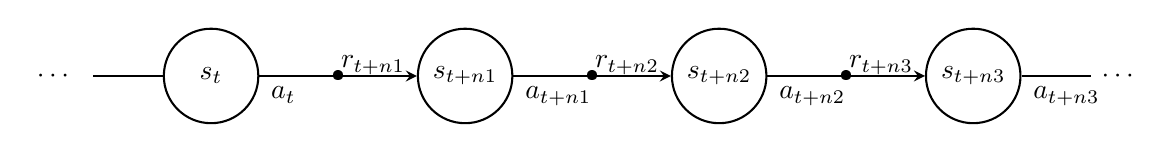
\begin{tikzpicture}[
                state/.style={circle, draw, minimum size=12mm},
                action/.style={text height=1.5ex, text depth=.25ex},
                reward/.style={text height=1.5ex, text depth=.25ex},
                every loop/.style={looseness=8},
                >=stealth
            ]
            
            % Nodes (States)
            \node[state] (s_t) {$s_t$};
            \node[state, right=2cm of s_t] (s_tn1) {$s_{t+n1}$};
            \node[state, right=2cm of s_tn1] (s_tn2) {$s_{t+n2}$};
            \node[state, right=2cm of s_tn2] (s_tn3) {$s_{t+n3}$};
            
            % Actions
            \node[action, below right=-0.5cm and 0.2cm of s_t] (a_t) {$a_t$};
            \node[action, below right=-0.5cm and 0.2cm of s_tn1] (a_tn1) {$a_{t+n1}$};
            \node[action, below right=-0.5cm and 0.2cm of s_tn2] (a_tn2) {$a_{t+n2}$};
            \node[action, below right=-0.5cm and 0.2cm of s_tn3] (a_tn3) {$a_{t+n3}$};
            
            % Rewards
            \node[reward, above left=-0.5cm and 0.2cm of s_tn1] (r_tn1) {$r_{t+n1}$};
            \node[reward, above left=-0.5cm and 0.2cm of s_tn2] (r_tn2) {$r_{t+n2}$};
            \node[reward, above left=-0.5cm and 0.2cm of s_tn3] (r_tn3) {$r_{t+n3}$};
            
            % State Transitions
            \draw[->] (s_t) -- (s_tn1) node[midway] {\textbullet};
            \draw[->] (s_tn1) -- (s_tn2) node[midway] {\textbullet};
            \draw[->] (s_tn2) -- (s_tn3) node[midway] {\textbullet};

            % Dots for continuation
            \draw (s_tn3) -- ++(1.5,0)[right=2cm of s_tn3] node (dots) {$\cdots$};
            \draw (s_t) -- ++(-1.5,0) node[left=1cm of s_t] (dots) {$\cdots$};
        \end{tikzpicture}
    \end{figure}
    \item Bellman Equation
        \begin{equation*}
            \begin{split}
                &V^*(s)=\max_{a\in A_{s}}\bigg[R(s,a)+\sum_{s',\tau}\gamma^\tau P(s',\tau|s,a)V^*(s')\bigg]\\
                &Q^*(s,a)=R(s,a)+\sum_{s',\tau}\gamma^\tau P(s',\tau|s,a)\max_{a'\in A_{s'}}Q^*(s',a')
            \end{split}
        \end{equation*}
    \item For SMDP, one-step Q-learning becomes
    \begin{equation*}
        Q(s_t,a_t)\gets Q(s_t,a_t)+\alpha[r_{t+\tau}+\gamma^\tau \max_{a}Q(s_{t+\tau},a)-Q(s_t,a_t)]
    \end{equation*}
    \item We can define three notions of optimality
    \item \textbf{Hierarchically Optimal} policies that give the best solution yet satisfies the proposed hierarchies
    \item \textbf{Recursive Optimal} policies are the best policies formed by putting together component-wise policies obtained by optimizing for each component.
    \item \textbf{Flat Optimal} policies are the same as a regular optimal policy that does not consider any hierarchy.
    \item \textbf{Options Framework}: A generalization of actions to include temporally-extended courses of actions, \url{https://people.cs.umass.edu/~barto/courses/cs687/Sutton-Precup-Singh-AIJ99.pdf}
    \item An option is a triple, $o=\langle I,\pi_o,\beta \rangle$
    \begin{enumerate}
        \item $I\subseteq S$ is the set of states in which $o$ may be started
        \item $\pi_o:\Psi \to[0,1]$ is the stochastic policy followed during $o$
        \item $\beta:S\to [0,1]$ is the probability of terminating in each state
    \end{enumerate}
    \item \textbf{Generalizing over tasks}: Each task has a different reward structure in the state space.
    \item Options provide a model for subtasks, semi Markov Process.
    \item Options help in transfer learning, long-term planning, and faster convergence in RL.
    \item We can use generalization of TD, Q-Learning, SARSA, etc. with options.
\end{itemize}

\subsection{Monte Carlo Tree Search}
\begin{itemize}
    \item In online planning, planning is undertaken immediately before executing an action. 
    \item Once an action (or perhaps a sequence of actions) is executed, we start planning again from the new state. 
    \item As such, planning and execution are interleaved such that:
    \begin{enumerate}
        \item For each state $s$ visited, the set of all available actions $A(s)$ are partially evaluated
        \item $Q(s,a)$ is approximated by averaging the expected reward of trajectories over $S$ obtained by repeated simulations.
        \item The chosen action is $\argmax_a Q(s,a)$.
    \end{enumerate}
    \item Consider the following tree representing a MDP, where black circles represent actions and white represent states.
    \begin{figure}[H]
        \centering
        \includegraphics[width=0.6\linewidth]{Degree//static/RL_MDP_tree.png}
        \caption{Tree Representing MDP}
    \end{figure}
    \item \textbf{Selection}: Start at the root node, and successively select a child until we reach a node that is not fully expanded.
    \begin{figure}[H]
        \centering
        \includegraphics[width=0.6\linewidth]{Degree//static/RL_MDP_tree_selection.png}
        \caption{Selection Process}
    \end{figure}
    \item \textbf{Expansion}: Expand the children of the selected node by choosing an action with selection policy or tree policy and creating new nodes using the action outcomes.
    \begin{figure}[H]
        \centering
        \includegraphics[width=0.6\linewidth]{Degree//static/RL_MDP_tree_expansion.png}
        \caption{Expansion Process}
    \end{figure}
    \item \textbf{Simulation}: Choose one of the new nodes and perform a random simulation of the MDP to the terminating state with rollout policy
    \begin{figure}[H]
        \centering
        \includegraphics[width=0.6\linewidth]{Degree//static/RL_MDP_tree_simulation.png}
        \caption{Simulation Process}
    \end{figure}
    \item \textbf{Backup}: Given the reward $r$ at the terminating state, backup the reward to calculate the value $Q(s,a)$ at each state along the path.
    \begin{figure}[H]
        \centering
        \includegraphics[width=0.6\linewidth]{Degree//static/RL_MDP_tree_backup.png}
        \caption{Backup Process}
    \end{figure}
    \begin{algorithm}[H]
        \caption{Monte Carlo Tree Search}
        \begin{algorithmic}[1]
            \Function{MCTSearch}{$s_0$}
                \While{within computational budget}
                    \State $selectedNode$ $\gets$ \Call{Select}{$s_0$}
                    \State $child$ $\gets$ \Call{Expand}{$selectedNode$}
                    \State $G$ $\gets$ \Call{Simulate}{$child$}
                    \State \Call{Backup}{$child$,$G$}
                \EndWhile
                \State \Return $\argmax_aQ(s_0,a)$
            \EndFunction
            \Statex
            \Function{Select}{$s$}
                \While{$s$ is fully expanded}
                    \State Select action $a$ to apply in $s$ according to tree policy
                    \State Get next state $s'$
                    \State $s\gets s'$
                \EndWhile
                \State \Return $s$
            \EndFunction
            \Statex
            \Function{Expand}{$s$}
                \State Select action $a$ to apply in $s$ according to tree policy
                \State Get next state $s'$ and reward $r$
            \EndFunction
            \Statex
            \Function{Backup}{$s$,$G$}
                \Repeat
                    \State $N(s,a)\gets N(s,a)+1$
                    \State $G\gets r+\gamma G$
                    \State $Q(s,a)\gets Q(s,a)+\frac{1}{N(s,a)}[G-Q(s,a)]$
                    \State $s\gets$ parent of $s$
                \Until{$s\neq s_0$}
            \EndFunction
        \end{algorithmic}
    \end{algorithm}
    \item \textbf{Aheuristic}: MCTS doesn't need domain-specific knowledge, making it readily applicable to any domain that may be modelled using a tree.
    \item \textbf{Asymmetric}: the tree selection allows the algorithm to focus on promising nodes, leading to an asymmetric tree expansion.
    \item \textbf{Anytime}: MCTS backups the outcome of each simulation immediately, which ensures all values are always up to-date following every iteration of the algorithm. This allows the algorithm to return an action from the root at any moment in time.
    \item \textbf{UCT}: Upper Confidence bound for Trees, UCB1 + MCTS
    \item The UCT selection strategy is similar to UCB1 selection strategy
    \begin{equation*}
        \argmax_{a\in A(s)}\bigg[Q(s,a)+2c\sqrt{\frac{2\ln{N(s)}}{N(s,a)}}\bigg]
    \end{equation*}
    \item $N(s)$: The number of times a state node has been visited
    \item $N(s,a)$: The number of times action $a$ has been selected from this node
    \item $c>0$ is the exploration constant
    \item A few applications for this include Alpha Go Zero, Chess, Shogi, Real Time Strategy games, and Planning and scheduling
\end{itemize}

\end{document}